\section{Funcionamiento de sensores de contacto } 
Dichos sensores poseen un switch que al entrar en contacto con una superficie, emite una señal eléctrica que activa o desactiva el paso de la energía. 
Al poseer una composición robusta,  es favorable para evitar choques al detener los actuadores. 

\section*{Ventajas}
\begin{itemize}
	\item Detección de objetos 
	\item  Prevención de choques  
	\item Automatización de procesos 
\end{itemize}


\section*{Aplicaciones de un sensor de contacto} 
\begin{itemize}
	\item Medición de fuerza y presión 
	\item Control de nivel líquido  
	\item Envío de señales de retorno 
	\item Control de posición de válvulas
\end{itemize}


\section{Giroscopio}
El giroscopio consiste en un sensor interno de posición que viene integrado en los dispositivos. Este permite al dispositivo conocer su orientación y posición en el espacio mediante tres sistemas integrados en el chip, cada uno jugando un rol en el eje “x”, “y” y “z” respectivamente.

En la imagen\autoref{fig:GIROSCOPIO} se puede observar 6 diferentes secciones del microchip. Las 3 partes superiores forman parte de un acelerómetro, mientras que las 3 partes inferiores son los tres sensores del giroscopio. Orientados de izquierda a derecha serían eje “z”, “x” y “x”.

\begin{figure}[h]
	\centering
	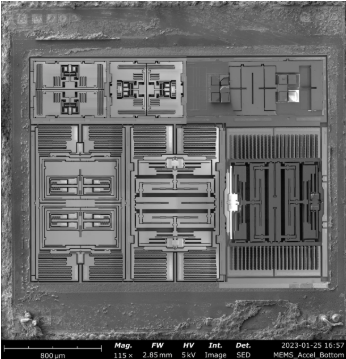
\includegraphics[width=0.3\linewidth]{img/GIROSCOPIO}
	\caption{Imagen de un Giroscopio  }
	\label{fig:GIROSCOPIO}
\end{figure}

Las partes de dirección  “x” y dirección “y” son básicamente la misma pieza pero rotada 90 grados. La parte direccional de “z” tiene una composición distinta a la de sus otras contrapartes.

El funcionamiento general del sistema utiliza un fenómeno conocido como efecto coriolis y algo parecido a la resonancia de un diapasón, ya que en conjunto de las fuerzas generadas por las vibraciones, las cuales hacen que dos piezas paralelas resuenen entre sí, más el efecto coriolis en la rotación, generando así una desviación en la frecuencia.


